%

Ciężko uniknąć sytuacji, w której systemy wykorzystujące do komunikacji standard \emph{802.11} napotykają potrzebę zmiany częstotliwości (przełączenia kanału) pracy swoich interfejsów kart radiowych NIC (ang. \emph{Network Interface Card}). Główną przyczyną podziału pasma jest wielodostęp, a więc unikanie wzajemnego zakłócania się urządzeń. Należy wziąć pod uwagę, że medium transmisyjne w środowisku przemysłowym jest zwykle wyjątkowo zaszumione w paśmie \emph{2.4 GHz}. Dla uzmysłowienia stopnia zakłóceń wystarczy wymienić część urządzeń pracujących w paśmie \emph{ISM} (ang. \emph{Industrial, scientific and medical}) takich jak:
\begin{itemize}
\item[--] elektroniczne nianie,
\item[--] urządzenia Bluetooth,
\item[--] kuchenki mikrofalowe,
\item[--] alarmy samochodowe
\end{itemize}
Łatwo zauważyć jak bardzo zróżnicowane urządzenia mogą doprowadzić do problemów w bezprzewodowej komunikacji systemów czasu rzeczywistego.

Warto wspomnieć, że istnieje już specyfikacja standardu pracującego w paśmie \emph{5 GHz} (\cite{std:IEEE80211n}), lecz nie jest on jeszcze powszechnie wspierany. Biorąc za przykład rozwiązania \emph{open-source} można zauważyć, że standard \emph{802.11n} jest obsługiwany przez nowe sterowniki (\emph{ath9k} dla urządzeń firmy \emph{Atheros}). Problemem jest natomiast fakt, że tego typu sterowniki dostępne są jedynie w najnowszych dystrybucjach systemów operacyjnych przeznaczonych dla urządzeń wbudowanych (przykładowo \emph{OpenWrt Backfire 10.03}), które nie zawsze od początku wspierają zadowalającą gamę urządzeń. Dla przykładu nadal istnieją problemy z dostępnością tego typu sterowników dla popularnej płytki \emph{MagicBox}.

Biorąc pod uwagę fakt zaszumienia medium transmisyjnego wnioskuję, że możliwość zmiany częstotliwości pracy interfejsu \emph{NIC} w poszukiwaniu dogodnego kanału komunikacji jest jedną z jego kluczowych i wymagających uwagi cech. W ostatnich latach powstało wiele publikacji dotyczących możliwości adaptacji struktury sieci bezprzewodowych do panującej jakości medium komunikacyjnego (\cite{pub:DCS}). Prace te koncentrują się głównie na algorytmach dynamicznej modyfikacji częstotliwości pracy interfejsów w sieciach kratowych \emph{WMN} (ang. \emph{Wireless Mesh Network}). Oczywiście u podstaw zastosowanych rozwiązań leży zjawisko przełączania kanału radiowego.

Powyższe czynniki sugerują, że całkowite wyeliminowanie potrzeby przełączania kanału (zmiany częstotliwości pracy) interfejsów radiowych nie jest aktualnie osiągalne. Co więcej, udostępnianie nowych pasm częstotliwości, w sytuacji ciągle rosnącego zapotrzebowania, jest jedynie tymczasowym rozwiązaniem.  


% Rozwiązanie z 2-3 interfejsami radiowymi ???
\section{Przełączanie kanału radiowego.}
Opóźnienie związane ze zmianą częstotliwości pracy jest ważnym parametrem, gdyż w tym czasie stacja zaprzestaje reakcji na kierowane do niej dane. Ramki skierowane do stacji są tracone co w oczywisty sposób może wpłynąć na ograniczenia czasowe, w których działają komunikujące się systemy. 
Typowe scenariusze, w których może zajść potrzeba zmiany częstotliwości pracy interfejsu NIC to:
\begin{itemize}
\item[--] Stacja kliencka w trybie \emph{Managed} dokonuje \emph{Roamingu} między dwoma punktami dostępowymi AP (ang. \emph{Access Point}) 
\item[--] Stacja kliencka w trybie \emph{Managed} skanuje medium w poszukiwaniu punktów dostępowych AP (ang. \emph{Access Point})
\item[--] Stacja kliencka w trybie \emph{Ad-hoc} skanuje medium po aktywacji interfejsu lub samym przełączeniu kanału 
\end{itemize}
Identyfikacja powyższych sytuacji to pierwszy krok ku specyfikacji konkretnych scenariuszy pomiarowych. 

Najczęstszą przyczyną przełączania kanału jest procedura skanowania medium komunikacyjnego. Podczas skanowania stacja wysyła ramki typu \emph{Probe Request} na każdej z dostępnych w specyfikacji (\cite{std:IEEE80211}) częstotliwości pracy i oczekuje na ramki \emph{Probe Response} od punktów dostępowych, lub stacji w trybie \emph{Ad-hoc} (w zależności od typu interfejsu NIC, czyli rodzaju docelowej sieci).

Przełączanie kanału następuje również, kiedy stacja kliencka oddala się zbyt daleko od punktu dostępowego i musi rozpocząć poszukiwanie nowego w swoim zasięgu. Jest to sytuacja zwana roamingiem i wymaga uwagi podczas rozważania systemów, w których skład wchodzą mobilne stacje, czy agenci. Obszar działania systemu może być na tyle różnorodny pod względem zakłóceń, że konieczne będzie przełączanie kanału między kolejnymi punktami dostępowymi pracującymi na różnych częstotliwościach.

\section{Metodyka pomiaru.}
Z punktu widzenia zjawiska komunikacji w standardzie 802.11 za kluczową uznałem możliwość prowadzenia pomiarów z minimalną ingerencją w strukturę i działanie stacji. Osiągnięcie tego celu wymaga uruchomienia dodatkowej maszyny, która prowadzi nasłuch w medium komunikacyjnym. Jedną z zalet tego typu rozwiązania jest fakt, że programistyczne środowisko pomiarowe przygotowuję tylko na jednej stacji. Jest to niezwykle ważne w przypadku, gdy w danym scenariuszu pomiarowym biorą udział systemy wbudowane (np. pełniące funkcję routerów) z ograniczonymi możliwościami instalacji rozbudowanych aplikacji i bibliotek programistycznych. 

Warto zauważyć, że stacje mogą pracować na różnych częstotliwościach i zmieniać je w trakcie trwania obserwacji. Stacja pomiarowa, będąca w posiadaniu informacji na temat aktualnie badanego zjawiska, musi mieć możliwość zmiany kanału pracy swojego interfejsu nasłuchującego w sposób, który nie spowoduje utraty informacji z łącza. Jednym z rozwiązań tego problemu jest zastosowanie wielu interfejsów radiowych, które podczas inicjalizacji procedury pomiarowej wprowadzane są na częstotliwości pracy przeznaczone do obserwacji konkretnych uczestników. 

Opis stosowanych metodyk pomiarowych rozpocznę od definicji podstawowych pojęć opisujących środowisko i uczestników scenariuszy. Najważniejsze pojęcia to:
\begin{itemize}
\item[--] {\bf Stacja pomiarowa}: Komputer działający pod kontrolą interakcyjnego systemu operacyjnego, na którym uruchomiona jest aplikacja nasłuchująca ruch sieciowy (ang. \emph{sniffer}).
\item[--] {\bf Stacja kliencka}: Komputer pełniący rolę klienta w sieci o strukturze wykorzystującej punkty dostępowe (ang. \emph{Infrastructure mode}). Może być to zarówno komputer pod kontrolą systemu interakcyjnego, lub wbudowanego.
\item[--] {\bf Punkt dostępowy}: Komputer pełniący w trybie infrastruktury (ang. \emph{Infrastructure mode}) rolę stacji AP (ang. \emph{Access Point}). Może być to zarówno komputer pod kontrolą systemu interakcyjnego, lub wbudowanego.
\item[--] {\bf Rozwiązanie asocjacji}: Zdarzenie wysłania ramki rozwiązującej asocjację między stacją kliencką, a punktem dostępowym (ang. \emph{Disassociation frame}).
\item[--] {\bf Skanowanie}: Wysyłanie przez stację ramek typu \emph{Probe Request} na wszystkich dostępnych w specyfikacji (\cite{std:IEEE80211}) częstotliwościach pracy.
\item[--] {\bf Scenariusz pomiaru}: Jeden ze scenariuszy możliwych do zaistnienia podczas komunikacji stacji w standardzie 802.11, w którego czasie następuje przełączenie kanału interfejsu NIC.
\item[--] {\bf Zdarzenie}: Przechwycenie ramki standardu 802.11 biorącej udział w scenariuszu pomiarowym. 
\end{itemize}

\section{Scenariusz pomiaru: Roaming 802.11.}
Roaming 802.11 to zjawisko zachodzące w sieciach, w trybie infrastruktury (ang. \emph{Infrastructure mode}). Podstawowym celem jest umożliwienie stacji klienckiej odłączenia się od punktu dostępowego i podjęcia próby odnalezienia i podłączenia się do stacji o mocniejszym sygnale. W warunkach rzeczywistych sytuacja taka najczęściej jest wynikiem ruchu mobilnej stacji klienckiej (np. przemieszczającego się pracownika biura, lub agenta w systemie przemysłowym), która dociera do granicy zasięgu dotychczas używanego punktu dostępowego. Aby zachować połączenie z systemem, lub usługami (np. dostęp do internetu) maszyna musi odnaleźć inną stację pracującą w trybie AP o mocniejszym sygnale. Na procedurę roamingu 802.11 składają się następujące kroki:
\begin{itemize}
\item[--] Stacja kliencka wykrywa, że poziom sygnału RF (ang. \emph{Radio Frequency})
punktu dostępowego \#1 jest poniżej progu roamingu.
\item[--] Stacja kliencka rozpoczyna nadawanie ramek rozwiązujących asocjację do punktu dostępowego \#1 do momentu potwierdzenia odebrania.
\item[--] Punkt dostępowy \#1 otrzymuje ramkę rozwiązującą asocjację \emph{Disassociation frame} i usuwa stację kliencką z tablicy asocjacji.
\item[--] Stacja kliencka rozpoczyna skanowanie medium komunikacyjnego i oczekuje ramek \emph{Probe Response}.
\item[--] Punkt dostępowy \#2 wysyła do stacji klienckiej ramkę typu \emph{Probe Response}.
\item[--] Stacja kliencka rozpoczyna wysyłanie do punktu dostępowego \#2 ramek typu \emph{Association request}.
\item[--] Punkt dostępowy \#2 dokonuje asocjacji stacji klienckiej i potwierdza to zdarzenie wysyłając ramkę typu \emph{Association response}.
\end{itemize}

Łatwo zauważyć, że zjawisko roamingu jest kluczowe w przypadku systemu czasu rzeczywistego zarządzającego stacjami mobilnymi na rozległym obszarze (\ref{MobileAgentSystem}). System może wykorzystywać wiele punktów dostępowych, które obsługuje poprzez sieć przewodową (ang. \emph{Ethernet}). Każda zarządzana stacja w trybie AP przystosowana jest do działania w panujących na swoim obszarze warunkach zaszumienia łącza. Roaming 802.11 byłby w tym wypadku główną przyczyną przełączania kanału radiowego interfejsu NIC w mobilnych stacjach klienckich. 

\begin{figure}[htb]
\begin{center}
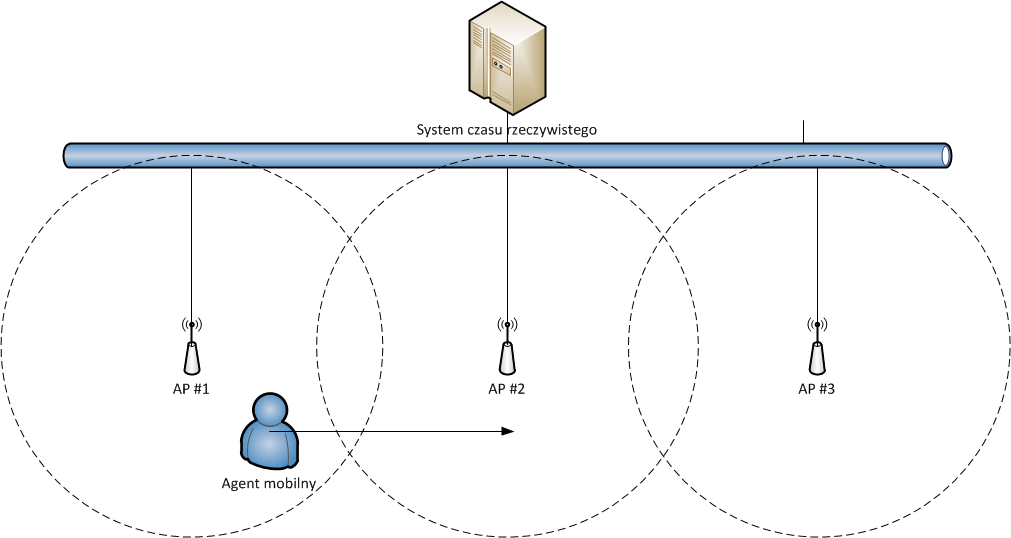
\includegraphics[width=250px]{img/System_czasu_rzeczywistego}
\caption{System z mobilnym agentem}
\label{MobileAgentSystem}
\end{center}
\end{figure}

Oczywiście roaming nie implikuje ruchu żadnej z maszyn, co ułatwia przeprowadzenie pomiaru. Wystarczy doprowadzić do sytuacji, w której moc sygnału punktu dostępowego spadnie poniżej progu (ang. \emph{roaming threshold}), który powoduje decyzję o rozwiązaniu asocjacji stacji klienckiej. 

\begin{figure}[htb]
\begin{center}
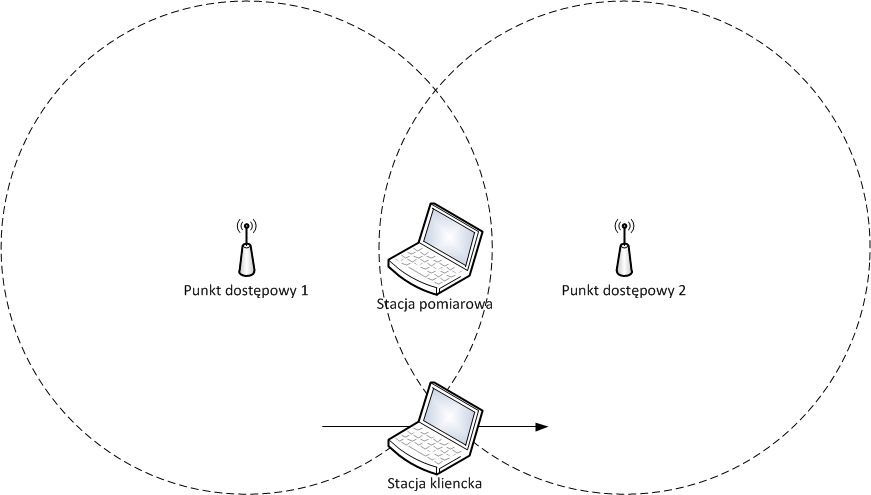
\includegraphics[width=250px]{img/Roaming}
\caption{Roaming 802.11: Środowisko pomiarowe.}
\label{RoamingEnviroment}
\end{center}
\end{figure}

\subsection{Środowisko pomiarowe.}
\label{sec:MeasurementEnviroment}

W skład środowiska pomiarowego (\ref{RoamingEnviroment}) wchodzą dwa punkty dostępowe, stacja kliencka oraz stacja pomiarowa. Punkty dostępowe pracują na różnych częstotliwościach. Do wyboru, zgodnie ze standardem 802.11g (\cite{std:IEEE80211}), są kanały numer 1, 5, 9, lub 13. Są to nienachodzące na siebie zakresy częstotliwości. W celu ułatwienia roamingu stacja kliencka umieszczona jest na granicy zasięgu punktów dostępowych. Stacja pomiarowa musi znajdować się w zasięgu stacji klienckiej, oraz obydwu punktów dostępowych (musi być w stanie rejestrować ruch sieciowy). 
Należy zwrócić uwagę na zapewnienie odpowiedniej jakości medium transmisyjnego. Wysoki poziom zakłóceń na kanałach wykorzystywanych w eksperymencie wprowadzi zakłamania, jeśli interesuje nas wyłącznie czas trwania samej procedury roamingu. 

\subsection{Mierzona wartość: Czas roamingu.}
Czas roamingu 802.11 rozumiem jako czas (\ref{RoamingTime}) mierzony od momentu decyzji stacji klienckiej o zaprzestaniu normalnej wymiany danych z punktem dostępowym do momentu powiązania z nową stacją w trybie AP o mocniejszym sygnale. Zdarzeniem inicjującym pomiar jest wysłanie przez stację kliencką pierwszej ramki rozwiązującej asocjację (ang. \emph{Disassociation frame}). Pomiar zostaje zakończony w momencie wysłania przez nowy punkt dostępowy ramki potwierdzającej asocjację nowej stacji (ang. \emph{Association Response frame}).

Podstawowa procedura pomiarowa składa się z następujących kroków:
\begin{itemize}
\item[--] Stacja kliencka przeprowadza asocjację z punktem dostępowym 1.
\item[--] Stacja kliencka przemieszcza się poza zasięg punktu dostępowego 1 i wykonuje procedurę roamingu do punktu dostępowego 2.
\item[--] Stacja pomiarowa wykrywa próbę rozwiązania asocjacji i rozpoczyna pomiar czasu.
\item[--] Punkt dostępowy 2 dokonuje asocjacji stacji klienckiej.
\item[--] Stacja pomiarowa rejestruje potwierdzenie asocjacji stacji klienckiej i zatrzymuje pomiar czasu.
\end{itemize}

\begin{figure}[htb]
\begin{center}
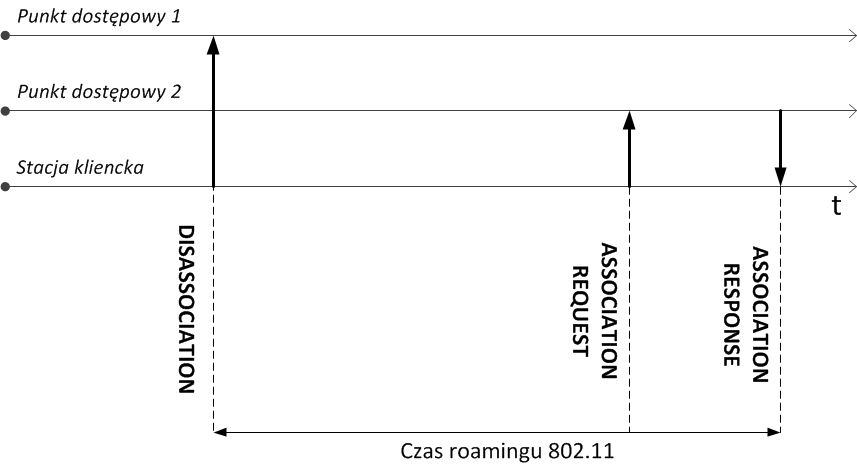
\includegraphics[width=250px]{img/RoamingTime}
\caption{Roaming 802.11: Czas roamingu.}
\label{RoamingTime}
\end{center}
\end{figure}

\subsection{Wymagania co do aplikacji \emph{hop-sniffer}.}
\label{sec:ApplicationRequirements}

Do przeprowadzenia powyżej zdefiniowanej procedury pomiaru opóźnienia roamingu stacji klienckiej niezbędne jest wytworzenie oprogramowania pomocniczego. Aplikacja ta działa w środowisku stacji pomiarowej i służy do przechwytywania i reagowania na zdarzenia scenariusza. Powinna ona spełniać wszelkie wymagania funkcjonalne i niefunkcjonalne stawiane przez procedurę pomiarową. W wyniku analizy zidentyfikowałem następujące wymagania: 
\begin{enumerate}
\item Architektura aplikacji nie jest rozproszona na wielu maszynach.
\item Aplikacja działa na komputerze przenośnym.
\item Aplikacja umożliwia przechwytywanie ramek zarządzających komunikacją standardu 802.11 (ang. \emph{Management}). 
\item Przechwytywane ramki muszą pochodzić z dowolnej sieci i adresów MAC (\emph{Media Access Control}).
\item Przechwytywanie musi odbywać się z minimalną ingerencją w badaną architekturę komunikacyjną.
\item Aplikacja przetwarza i buduje swoją logikę działania na podstawie zawartości nagłówków i pól danych pakietów. 
\item Dokładność pomiaru czasu musi być większa od interwałów występowania zdarzeń standardu 802.11.
\item Pomiar czasu musi być wykonany w zdefiniowanym momencie na określonym poziomie modelu stosu \emph{TCP/IP}.
\end{enumerate}

Scentralizowana architektura aplikacji oznacza działanie jej składników wyłącznie na stacji pomiarowej. Oznacza to, że wszelkie biblioteki i narzędzia programistyczną muszą być dostępne tylko na jednej maszynie. Ułatwia to przeprowadzenie pomiaru z udziałem dowolnych stacji (np. systemów wbudowanych uniemożliwiających instalację własnego oprogramowania). Eliminacji ulega również dodatkowy i ciężki do oszacowania narzut związany z komunikacją elementów samego systemu pomiarowego.

Działanie na komputerze przenośnym jest podyktowane łatwą organizacją określonego w specyfikacji środowiska. Stacja pomiarowa musi znajdować się w zasięgu wszystkich uczestników obserwowanego scenariusza, więc możliwa powinna być łatwa manipulacja jej położeniem.

Obserwacja opóźnień dowolnego zjawiska w standardzie 802.11 wymaga dostępu do elementarnych zdarzeń sterujących jego przebiegiem. Pochodną tego wymagania jest potrzeba nasłuchiwania w medium transmisyjnym w celu przechwytywania nie tyle ramek danych, co ramek porządkujących cały proces komunikacji (ang. \emph{Management frames}). Za ich pomocą stacje informują innych uczestników protokołu komunikacyjnego o rozpoczęciu, przebiegu i zakończeniu roamingu i innych opisanych w standardzie zjawisk. 

Niezwykle ważna jest konieczność obejścia dwóch niskopoziomowych filtrów pakietów, które stoją na przeszkodzie obserwacji wszystkich zdarzeń. Filtry te służą zwiększeniu wydajności komunikacji poprzez wczesne odrzucenie pakietów, które z pewnością nie interesują danej stacji. Pierwszym z nich jest filtr adresów \emph{MAC}, który odrzuca wszystkie ramki nie kierowane do danego interfejsu. Kolejnym jest filtr identyfikatorów \emph{SSID} (ang. \emph{Service Set Indetifier}), który upuszcza pakiety nie pochodzące z infrastruktury, której stacja nie jest członkiem. Stacja pomiarowa nie powinna być w asocjacji z żadnym punktem dostępowym, ale być w stanie przechwycić komunikaty pochodzące z dowolnego \emph{AP} (ang. \emph{Access Point}). 

Wymaganie co do minimalnej ingerencji w środowisko pomiarowe wynika z charakteru medium transmisyjnego. Interfejs stacji pomiarowej nie powinien pracować w żadnym trybie, który implikuje okresowe rozsyłanie ramek (przykładowo ramki typu \emph{Beacon} dla trybu \emph{AP}). Stacja nie powinna również podejmować prób asocjacji z punktami dostępowymi biorącymi udział w eksperymencie, aby nie wprowadzać dodatkowych opóźnień w pracy ich oprogramowania. Dopuszczalne jest rozesłanie ramek \emph{Probe Request} w fazie inicjalizacji środowiska w celu rozpoznania warunków panujących w medium transmisyjnym (moc nadawania, częstotliwości pracy poszczególnych interfejsów \emph{NIC}). 

Aplikacja działa na zasadzie reakcji na wartości odczytane z pól nagłówków i danych przechwyconych ramek. Powinna różnicować swoje zachowanie w zależności od tych informacji w celu realizacji zadanego scenariusza pomiarowego.

Dokładność pomiaru czasu przez aplikację \emph{hop-sniffer} musi być większa od podstawowej jednostki czasu używanej do określania interwałów czasu w standardzie 802.11. Jednostką tą jest TU (ang. \emph{Time Unit}) o długości 1024 mikrosekund. Specyfikacja taka wynika z potrzeby uniknięcia stosowania milisekund trudniejszych do odmierzenia w systemach mikroprocesorowych. Przyjmuję, że dokładność rzędu mikrosekund jest wystarczająca. Rząd milisekund może być nieodpowiedni ze względu na problem ze śledzeniem jednostki TU. Milisekunda nie mieści się w dowolnej mierze określonej w TU całkowitą liczbę razy. 

Aplikacja mierzy czas między zdarzeniami zdefiniowanymi jako fakt odebrania ramki określonego typu. Moment wystartowania licznika, bądź zebrania stempla czasowego na drodze ramki przez stos \emph{TCP/IP} powinien być jasno określony. Jeśli stacja pomiarowa działa pod kontrolą systemu operacyjnego pracującego w sposób niedeterministyczny to można spodziewać się trudnych w oszacowaniu opóźnień podczas uruchamiania licznika w warstwie aplikacyjnej.  



